\documentclass[]{article}
\usepackage{lmodern}
\usepackage{amssymb,amsmath}
\usepackage{ifxetex,ifluatex}
\usepackage{fixltx2e} % provides \textsubscript
\ifnum 0\ifxetex 1\fi\ifluatex 1\fi=0 % if pdftex
  \usepackage[T1]{fontenc}
  \usepackage[utf8]{inputenc}
\else % if luatex or xelatex
  \ifxetex
    \usepackage{mathspec}
  \else
    \usepackage{fontspec}
  \fi
  \defaultfontfeatures{Ligatures=TeX,Scale=MatchLowercase}
\fi
% use upquote if available, for straight quotes in verbatim environments
\IfFileExists{upquote.sty}{\usepackage{upquote}}{}
% use microtype if available
\IfFileExists{microtype.sty}{%
\usepackage{microtype}
\UseMicrotypeSet[protrusion]{basicmath} % disable protrusion for tt fonts
}{}
\usepackage[margin=1in]{geometry}
\usepackage{hyperref}
\hypersetup{unicode=true,
            pdftitle={Regression Models Course Project},
            pdfauthor={Sheila Braun},
            pdfborder={0 0 0},
            breaklinks=true}
\urlstyle{same}  % don't use monospace font for urls
\usepackage{color}
\usepackage{fancyvrb}
\newcommand{\VerbBar}{|}
\newcommand{\VERB}{\Verb[commandchars=\\\{\}]}
\DefineVerbatimEnvironment{Highlighting}{Verbatim}{commandchars=\\\{\}}
% Add ',fontsize=\small' for more characters per line
\usepackage{framed}
\definecolor{shadecolor}{RGB}{248,248,248}
\newenvironment{Shaded}{\begin{snugshade}}{\end{snugshade}}
\newcommand{\KeywordTok}[1]{\textcolor[rgb]{0.13,0.29,0.53}{\textbf{#1}}}
\newcommand{\DataTypeTok}[1]{\textcolor[rgb]{0.13,0.29,0.53}{#1}}
\newcommand{\DecValTok}[1]{\textcolor[rgb]{0.00,0.00,0.81}{#1}}
\newcommand{\BaseNTok}[1]{\textcolor[rgb]{0.00,0.00,0.81}{#1}}
\newcommand{\FloatTok}[1]{\textcolor[rgb]{0.00,0.00,0.81}{#1}}
\newcommand{\ConstantTok}[1]{\textcolor[rgb]{0.00,0.00,0.00}{#1}}
\newcommand{\CharTok}[1]{\textcolor[rgb]{0.31,0.60,0.02}{#1}}
\newcommand{\SpecialCharTok}[1]{\textcolor[rgb]{0.00,0.00,0.00}{#1}}
\newcommand{\StringTok}[1]{\textcolor[rgb]{0.31,0.60,0.02}{#1}}
\newcommand{\VerbatimStringTok}[1]{\textcolor[rgb]{0.31,0.60,0.02}{#1}}
\newcommand{\SpecialStringTok}[1]{\textcolor[rgb]{0.31,0.60,0.02}{#1}}
\newcommand{\ImportTok}[1]{#1}
\newcommand{\CommentTok}[1]{\textcolor[rgb]{0.56,0.35,0.01}{\textit{#1}}}
\newcommand{\DocumentationTok}[1]{\textcolor[rgb]{0.56,0.35,0.01}{\textbf{\textit{#1}}}}
\newcommand{\AnnotationTok}[1]{\textcolor[rgb]{0.56,0.35,0.01}{\textbf{\textit{#1}}}}
\newcommand{\CommentVarTok}[1]{\textcolor[rgb]{0.56,0.35,0.01}{\textbf{\textit{#1}}}}
\newcommand{\OtherTok}[1]{\textcolor[rgb]{0.56,0.35,0.01}{#1}}
\newcommand{\FunctionTok}[1]{\textcolor[rgb]{0.00,0.00,0.00}{#1}}
\newcommand{\VariableTok}[1]{\textcolor[rgb]{0.00,0.00,0.00}{#1}}
\newcommand{\ControlFlowTok}[1]{\textcolor[rgb]{0.13,0.29,0.53}{\textbf{#1}}}
\newcommand{\OperatorTok}[1]{\textcolor[rgb]{0.81,0.36,0.00}{\textbf{#1}}}
\newcommand{\BuiltInTok}[1]{#1}
\newcommand{\ExtensionTok}[1]{#1}
\newcommand{\PreprocessorTok}[1]{\textcolor[rgb]{0.56,0.35,0.01}{\textit{#1}}}
\newcommand{\AttributeTok}[1]{\textcolor[rgb]{0.77,0.63,0.00}{#1}}
\newcommand{\RegionMarkerTok}[1]{#1}
\newcommand{\InformationTok}[1]{\textcolor[rgb]{0.56,0.35,0.01}{\textbf{\textit{#1}}}}
\newcommand{\WarningTok}[1]{\textcolor[rgb]{0.56,0.35,0.01}{\textbf{\textit{#1}}}}
\newcommand{\AlertTok}[1]{\textcolor[rgb]{0.94,0.16,0.16}{#1}}
\newcommand{\ErrorTok}[1]{\textcolor[rgb]{0.64,0.00,0.00}{\textbf{#1}}}
\newcommand{\NormalTok}[1]{#1}
\usepackage{graphicx,grffile}
\makeatletter
\def\maxwidth{\ifdim\Gin@nat@width>\linewidth\linewidth\else\Gin@nat@width\fi}
\def\maxheight{\ifdim\Gin@nat@height>\textheight\textheight\else\Gin@nat@height\fi}
\makeatother
% Scale images if necessary, so that they will not overflow the page
% margins by default, and it is still possible to overwrite the defaults
% using explicit options in \includegraphics[width, height, ...]{}
\setkeys{Gin}{width=\maxwidth,height=\maxheight,keepaspectratio}
\IfFileExists{parskip.sty}{%
\usepackage{parskip}
}{% else
\setlength{\parindent}{0pt}
\setlength{\parskip}{6pt plus 2pt minus 1pt}
}
\setlength{\emergencystretch}{3em}  % prevent overfull lines
\providecommand{\tightlist}{%
  \setlength{\itemsep}{0pt}\setlength{\parskip}{0pt}}
\setcounter{secnumdepth}{0}
% Redefines (sub)paragraphs to behave more like sections
\ifx\paragraph\undefined\else
\let\oldparagraph\paragraph
\renewcommand{\paragraph}[1]{\oldparagraph{#1}\mbox{}}
\fi
\ifx\subparagraph\undefined\else
\let\oldsubparagraph\subparagraph
\renewcommand{\subparagraph}[1]{\oldsubparagraph{#1}\mbox{}}
\fi

%%% Use protect on footnotes to avoid problems with footnotes in titles
\let\rmarkdownfootnote\footnote%
\def\footnote{\protect\rmarkdownfootnote}

%%% Change title format to be more compact
\usepackage{titling}

% Create subtitle command for use in maketitle
\newcommand{\subtitle}[1]{
  \posttitle{
    \begin{center}\large#1\end{center}
    }
}

\setlength{\droptitle}{-2em}

  \title{Regression Models Course Project}
    \pretitle{\vspace{\droptitle}\centering\huge}
  \posttitle{\par}
    \author{Sheila Braun}
    \preauthor{\centering\large\emph}
  \postauthor{\par}
      \predate{\centering\large\emph}
  \postdate{\par}
    \date{July 3, 2018}


\begin{document}
\maketitle

\subsection{Executive Summary}\label{executive-summary}

This report relates to the mtcars data set. It contains linear modeling
analysis and responses to the following:

\begin{itemize}
\item
  \textbf{Is an automatic or manual transmission better for MPG?} As of
  1974 manaul transmissions were better for MPG than automatic
  transmissions.
\item
  \textbf{Quantify the MPG difference between automatic and manual
  transmissions}. Going from an automatic (am = 0) to a manual
  transmission (am = 1) increases \textbf{mpg} by 11.9385, unless the
  car also becomes heavier by half a ton, in which case mpg actually
  goes down, this time by 4.1974. Since 4.1974 (loss from getting a
  heavier car) is less than 11.9385 (gain from switching to a manual),
  it would still be worth getting a manual transmission even if it made
  your car heavier--at least in 1974.
\end{itemize}

The final model, detailed below, accounts for .8588 of the variance
(adjusted \emph{R} squared) with a \emph{p} value that is basically 0.

\subsection{Data}\label{data}

The data come from Henderson and Velleman (1981), Building multiple
regression models interactively. Biometrics, 37, 391--411. They are
collected into a data frame with 32 observations on 11 (numeric)
variables. The following table is a summary of the data.

\begin{verbatim}
##       mpg        cyl         disp             hp             drat      
##  Min.   :10.40   4:11   Min.   : 71.1   Min.   : 52.0   Min.   :2.760  
##  1st Qu.:15.43   6: 7   1st Qu.:120.8   1st Qu.: 96.5   1st Qu.:3.080  
##  Median :19.20   8:14   Median :196.3   Median :123.0   Median :3.695  
##  Mean   :20.09          Mean   :230.7   Mean   :146.7   Mean   :3.597  
##  3rd Qu.:22.80          3rd Qu.:326.0   3rd Qu.:180.0   3rd Qu.:3.920  
##  Max.   :33.90          Max.   :472.0   Max.   :335.0   Max.   :4.930  
##        wt             qsec       vs             am     gear   carb  
##  Min.   :1.513   Min.   :14.50   V:18   automatic:19   3:15   1: 7  
##  1st Qu.:2.581   1st Qu.:16.89   S:14   manual   :13   4:12   2:10  
##  Median :3.325   Median :17.71                         5: 5   3: 3  
##  Mean   :3.217   Mean   :17.85                                4:10  
##  3rd Qu.:3.610   3rd Qu.:18.90                                6: 1  
##  Max.   :5.424   Max.   :22.90                                8: 1
\end{verbatim}

See \emph{Figure 1} in the appendix for an initial look at the
relationships among the variables. On the face of it, \textbf{mpg} and
\textbf{am} (automatic vs.~manual transmission) have a linear
relationship. However \textbf{mpg} has interesting relationships with
all the variables with the possible exceptions of \textbf{gear} and
\textbf{qsec}. We must look at other variables that may affect
\textbf{mpg} and at any interaction terms in order to understand
thoroughly the relationship between \textbf{mpg} and \textbf{am}.

\subsubsection{Check Assumptions}\label{check-assumptions}

Linear regression modeling relies on normal data for accurate results.
See the appendix, Figures 2 and 3, for a histogram and qqplot of
\textbf{mpg}. Neither of them looks like a lovely normal distribution
should, but given a Shapiro-Wilk normality test with a p-value of
0.1228814, for now we fail to reject the null hypothesis that
\textbf{mpg} is normally distributed, bearing in mind that nevertheless
the data are less normally distributed than is ideal.

\subsection{Early Models}\label{early-models}

First, examine \textbf{mpg} as dependent variable with everything else
as predictors. In this initial model, the adjusted \emph{R} squared is
high at 0.8066423 and the overall p-value is quite low at 0.0000004. An
anova reveals three significant predictors: \textbf{cyl}, \textbf{disp},
and \textbf{wt}. The variable \textbf{am} is not significant in this
model, but it is our variable of interest and it has a known linear
relationship with \textbf{mpg} (see Figure 1 in the appendix), so this
model is suspect.

The second model is similar to the first one but the two variables
suspected of having little or no linear relationship with \textbf{mpg},
that is, \textbf{gear} and \textbf{qsec}, are no longer in the model.
Model 2's p-value is 0 and the adjusted \emph{R} squared is higher than
Model 1's at 0.8118215. An anova shows significant influences of
\textbf{cyl}, \textbf{disp}, and \textbf{wt} again. This model shows
that we can safely exclude \textbf{gear} and \textbf{qsec}.

The focus of the third model was to finalize a predictor list without
considering any interactions. That the variables \textbf{cyl},
\textbf{disp}, and \textbf{wt} belong in the model is possible based on
results of models 1 and 2. The variable \textbf{hp} correlates so highly
with cyl (\emph{r} = 0.8324475; \emph{p} = 0) that it might be possible
to leave it out while including \textbf{cyl}. Similarly, \textbf{cyl}
and \textbf{disp} are not only theoretically related, but their
correlation is even higher (\emph{r} = 0.9020329; \emph{p} = 0). Keeping
\textbf{cyl} in the model makes sense, and dropping \textbf{disp} from
the model also makes sense. Weight stays in because it is theoretically
different from the number of cylinders or automatic vs.~manual
transmission and because it has shown as a strong predictor in earlier
models. The variables \textbf{drat} and \textbf{am} correlate highly and
could be accounting for the same phenomenon (\emph{r} = 0.7127111;
\emph{p} = 0.0000047); we are interested in \textbf{am}, so we drop
\textbf{drat}. The variables \textbf{qsec} and \textbf{gear} are already
out of the model. The number of carburetors (\textbf{carb}) is another
variable that correlates highly with \textbf{hp} (\emph{r} = 0.7498125;
\emph{p} = 0.0000008) but not so much with the heretofore \textbf{hp}
proxy, \textbf{cyl} (\emph{r} = 0.5269883; \emph{p} = 0.0019423). For
that reason, we will put \textbf{hp} back in and leave \textbf{carb} out
rather than just putting \textbf{carb} in. We do not have any reason to
leave out \textbf{vs}, so it will also be in the model.

Model 3 accounts for a respectable 0.8228405 of the total variance in
\textbf{mpg} and it has a \emph{p} value of 0. The fact that the model
acounts for more variance than our previous best model, despite having
fewer variables, is encouraging.

\subsection{Final Model}\label{final-model}

By way of creating a final model, I looked carefully at all the other
models and the correlations to arrive at a final predictor list. This
model contains a possible interaction term, weight x automatic
vs.~manual transmission. In addition, I dropped \textbf{hp} and
\textbf{vs} because they performed poorly in early models.

\begin{Shaded}
\begin{Highlighting}[]
\NormalTok{fit5 <-}\StringTok{ }\KeywordTok{lm}\NormalTok{(mpg }\OperatorTok{~}\StringTok{ }\NormalTok{wt }\OperatorTok{+}\StringTok{ }\NormalTok{cyl }\OperatorTok{+}\StringTok{ }\NormalTok{am }\OperatorTok{+}\StringTok{ }\NormalTok{am }\OperatorTok{*}\StringTok{ }\NormalTok{wt, mtcars)}
\KeywordTok{summary}\NormalTok{(fit5)}
\end{Highlighting}
\end{Shaded}

\begin{verbatim}
## 
## Call:
## lm(formula = mpg ~ wt + cyl + am + am * wt, data = mtcars)
## 
## Residuals:
##     Min      1Q  Median      3Q     Max 
## -3.4621 -1.4913 -0.7879  1.3959  5.3499 
## 
## Coefficients:
##             Estimate Std. Error t value         Pr(>|t|)    
## (Intercept)  34.2830     2.7965  12.259 0.00000000000152 ***
## wt           -2.3689     0.8244  -2.874          0.00782 ** 
## cyl          -1.1814     0.3803  -3.106          0.00442 ** 
## am           11.9385     3.8453   3.105          0.00444 ** 
## wt:am        -4.1974     1.3115  -3.200          0.00350 ** 
## ---
## Signif. codes:  0 '***' 0.001 '**' 0.01 '*' 0.05 '.' 0.1 ' ' 1
## 
## Residual standard error: 2.265 on 27 degrees of freedom
## Multiple R-squared:  0.877,  Adjusted R-squared:  0.8588 
## F-statistic: 48.13 on 4 and 27 DF,  p-value: 0.000000000006643
\end{verbatim}

According to this model, mean miles per gallon is 34 when holding all
other variables equal. However, for every half ton of weight,
\textbf{mpg} goes down by 2.3689. Every 2 cylinders further reduces
\textbf{mpg} by 1.1814. Going from an automatic (am = 0) to a manual
transmission (am = 1) increases \textbf{mpg} by 11.9385, unless the car
also becomes heavier by half a ton, in which case \textbf{mpg} again
goes down, this time by 4.1974. Because the loss of \textbf{mpg} per
extra half ton is less than the gain in \textbf{mpg} due to switching to
a manual transmission, it would still be worth making the switch, at
least in terms of miles per gallon--and in 1974. See Figure 3 and 4 in
the appendix.

\pagebreak

\subsection{Appendix}\label{appendix}

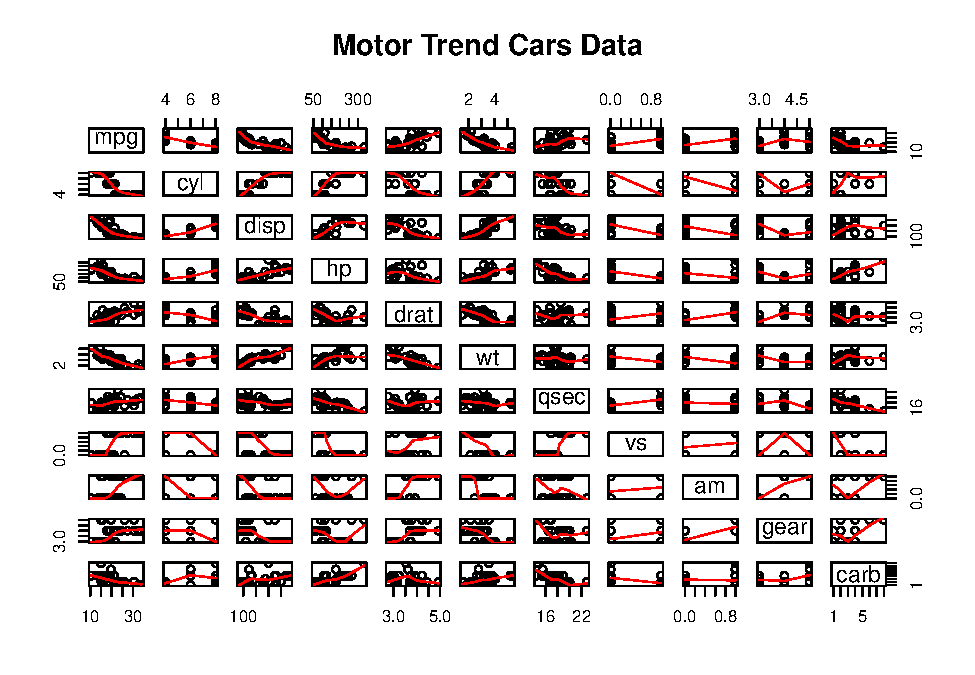
\includegraphics{Regression_Models_Course_Project_files/figure-latex/unnamed-chunk-2-1.pdf}

\emph{Figure 1.} Initial look at relationships among variables.

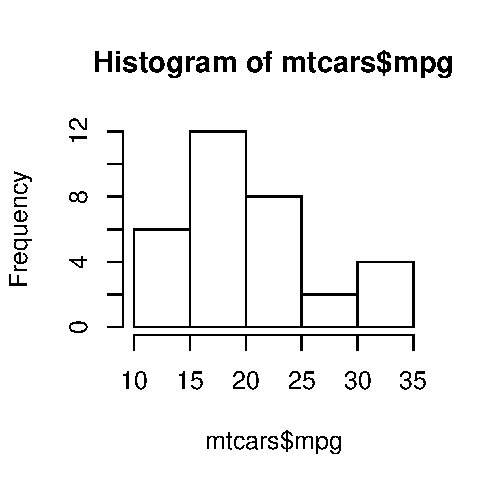
\includegraphics{Regression_Models_Course_Project_files/figure-latex/unnamed-chunk-3-1.pdf}
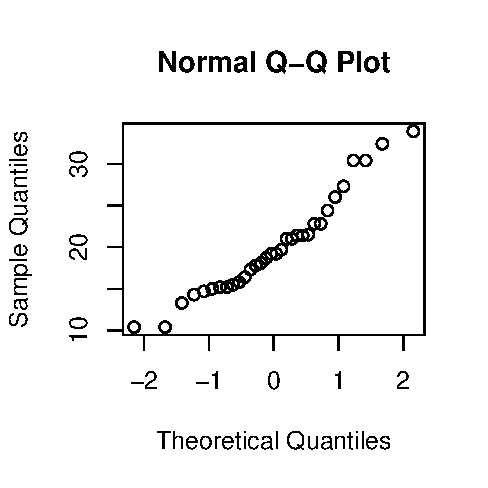
\includegraphics{Regression_Models_Course_Project_files/figure-latex/unnamed-chunk-3-2.pdf}

\emph{Figure 2.} Normality tests for \textbf{mpg}.

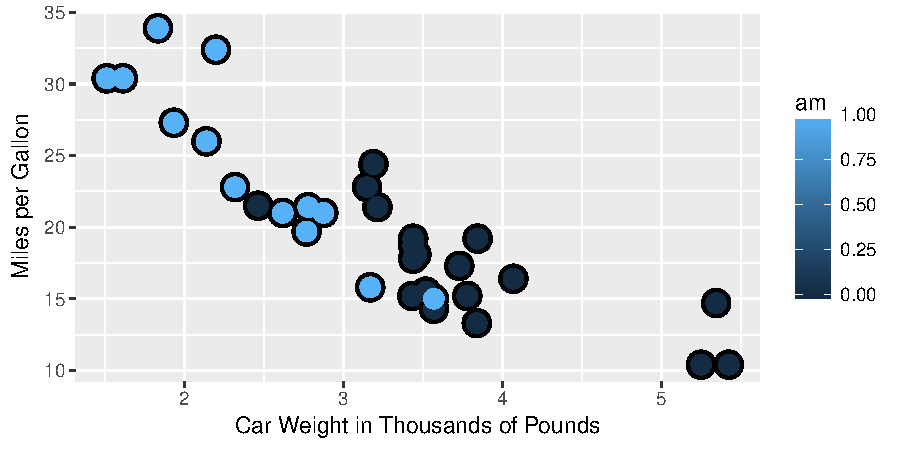
\includegraphics{Regression_Models_Course_Project_files/figure-latex/morePlots-1.pdf}

\emph{Figure 3.} The relationship between \textbf{mpg}, \textbf{weight},
and \textbf{am}.

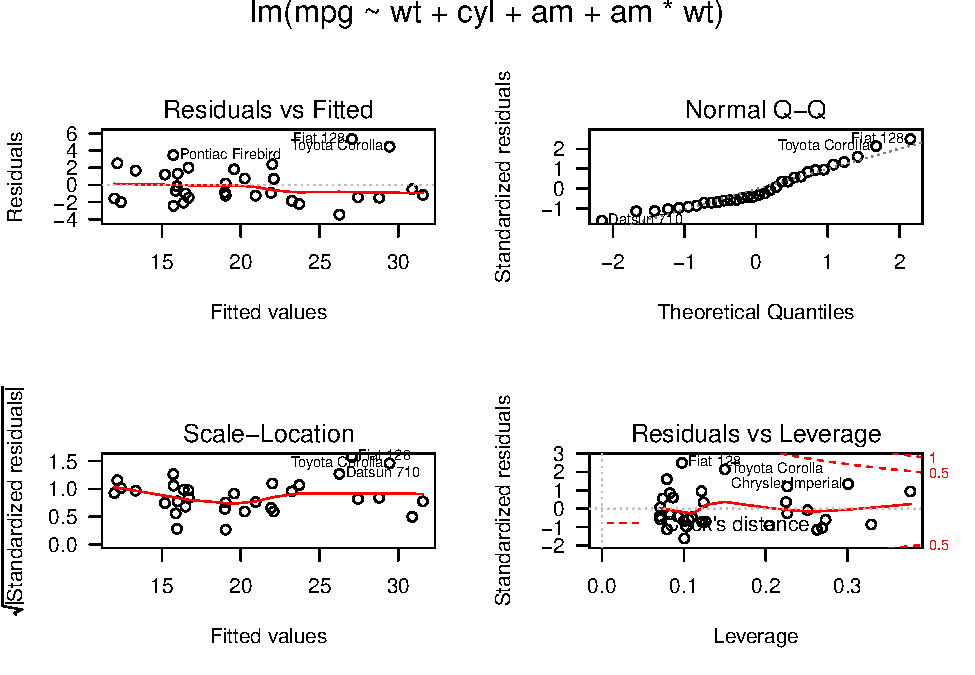
\includegraphics{Regression_Models_Course_Project_files/figure-latex/residual_plots-1.pdf}

\emph{Figure 4}. Diagnostic plots.


\end{document}
